\section{Experiments}\label{sec:experiments}
We evaluate three aspects of the approach: full-task composition, retention during sequential learning, and intermediate feedback. SmolVLA experiments test the adaptation pipeline in CDPR simulation. OpenVLA-OFT experiments test reward design on the ten LIBERO-Spatial tasks. The ongoing WX200 study examines another embodiment.

\subsection{SmolVLA: Complete-Task Adaptation}\label{sec:cdpr_results}
The CDPR simulation uses MuJoCo Warp/MJ-Lab, four object categories (apple, orange, potato, and tomato), and plate or bowl destinations. The action interface controls Cartesian translation, yaw, and the gripper. Strict success requires grasp, held lift, intentional release, and correct placement, without carry slip or wrong-placement events.

Separate evaluation covers 512 development scenes with four repeats each, excluding the in-run validation panel. Each attempt starts with an empty gripper and uses one full-task instruction, without teacher assistance. A later continuation supplies only TensorBoard in-run validation, with 1,024 attempts per reading. These two protocols are reported separately. All attempts, including numerical failures, remain in their respective denominators.
\subsection{Complete-Task Execution}
The adapted SmolVLA controller completes 1,258 of 2,048 attempts (61.43\%) from empty-gripper starts. Table~\ref{tab:cdpr} reports its task outcomes. Held lift occurs in 85.89\% of attempts, but only 71.52\% of held-lift attempts reach strict completion. Transport and release remain a major bottleneck. Plate and bowl completion rates are 68.58\% and 54.22\%, respectively. These are development results from one training lineage.
\begin{table}[t]
\caption{CDPR complete-task results at the 60.03M-action endpoint. Rates use all 1,024 attempts: 512 plate and 512 bowl episodes. Event flags can overlap.}
\label{tab:cdpr}\centering\small
\begin{tabular}{@{}lr@{}}\toprule
Outcome & Attempts (\%)\\\midrule
Physical grasp & 92.48\\
Held lift & 88.28\\
Strict completion (723/1,024) & 70.61\\
Carry slip & 16.70\\
Wrong placement & 14.16\\
Numerical failure & 0.88\\\bottomrule
\end{tabular}
\end{table}


\subsection{Base-Policy Skill Learning and Retention}\label{sec:skill_retention}
These measurements concern dense-reward training of simple CDPR skills and their consolidation into a base policy, before full-task composition. Each skill uses the instruction and reset protocol in Section~\ref{sec:skill_acquisition}; placement tests start with the object already held. Learning a new skill can degrade previously learned behavior, although the same policy must retain all component skills to execute the complete multi-stage task.

\begin{figure*}[!t]
\centering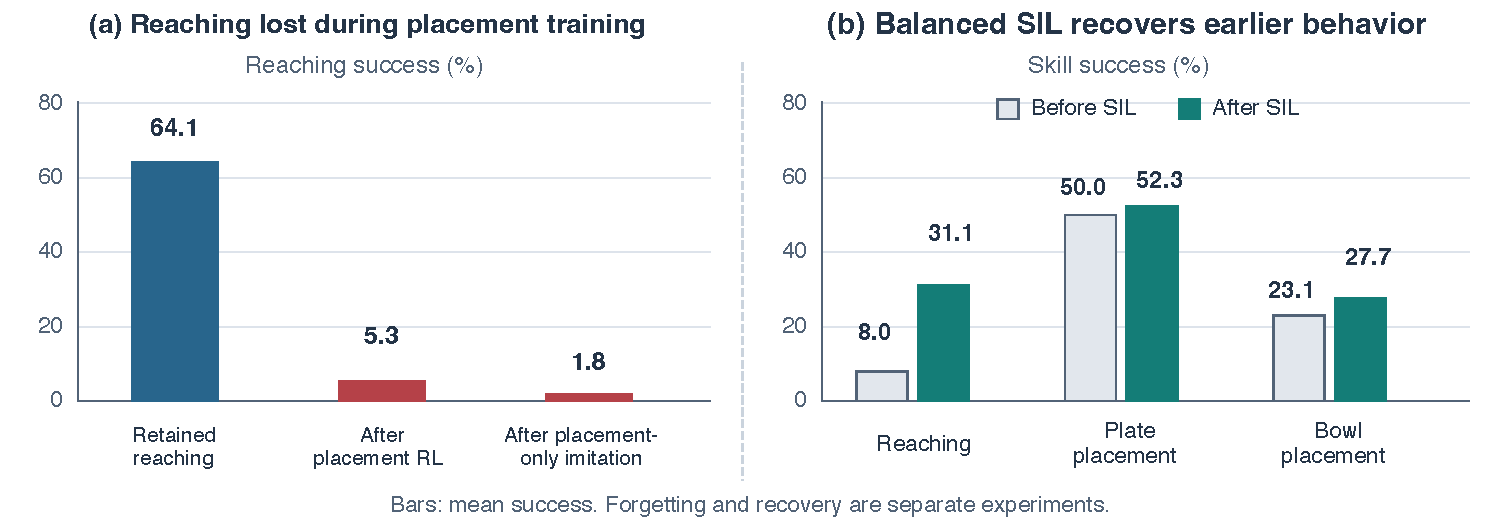
\includegraphics[width=\textwidth]{figures/skill_retention.pdf}
\caption{Base-policy skill recovery before full-task composition. Bars show means and points show individual evaluation rounds: three for reaching and two for each placement skill, per condition. Reaching uses the instruction \emph{move to \textless object\textgreater}; placement starts with the object already held. Reaching partially recovers while both placement means increase.}
\label{fig:retention}
\end{figure*}

In a forgetting evaluation, mean reaching success falls from 64.1\% for the reaching reference to 5.3\% after placement RL, over three evaluation rounds per condition. The recovery evaluation in Fig.~\ref{fig:retention} is a separate measurement: balanced self-imitation raises reaching success from 8.0\% to 31.1\%. Plate placement changes from 50.0\% to 52.3\%, and bowl placement from 23.05\% to 27.65\%. The bank combines earlier reaching successes with current placement successes, balancing the retained data by instruction.

Recovery is partial, with placement performance retained while reaching improves. Table~\ref{tab:skill_matrix} summarizes skill-specific RL references and a shared policy after subsequent consolidation. Evaluation reset distributions differ across stages. The shared policy succeeds on all four skills, although pickup remains weak. These skill evaluations do not isolate the contribution of self-imitation to final full-task success.

% Reaching reference: evidence/skill_retention_rounds.json, forgetting comparison.
% Other rows: ../CDPR_CONSOLIDATED_PROGRESS_REPORT.md, instruction success table;
% consolidation is the Cycle 3 shared policy, evaluated before composition.
\begin{table}[!ht]
\caption{Skill success (\%) by training stage. Placement starts with the object held; --- denotes an unreported result.}
\label{tab:skill_matrix}\centering\small
\begin{tabular}{@{}lrrrr@{}}\toprule
Training stage & Reach & Pickup & Plate & Bowl\\\midrule
Reaching RL & 64.1 & --- & --- & ---\\
Pickup RL & --- & 26.0 & --- & ---\\
Placement RL & --- & --- & 71.0 & 32.0\\
After consolidation & 47.8 & 11.9 & 73.8 & 53.5\\\bottomrule
\end{tabular}
\end{table}



\subsection{Intermediate Feedback on LIBERO-Spatial}\label{sec:libero_results}
This experiment compares feedback for complete manipulation instructions, using OpenVLA-OFT and SimpleVLA-RL to hold the backbone and training framework fixed across reward conditions~\cite{openvlaoft,simplevlarl}. It tests an ingredient of the adaptation pipeline; the complete training schedule is evaluated on the CDPR.

We fine-tune with LoRA on the ten LIBERO-Spatial tasks~\cite{libero}, using the feedback variants in Section~\ref{sec:composition}. All runs share a 61.0\% initialization and use 300 validation rollouts per endpoint. The terminal-only baseline is trained with SimpleVLA-RL under the same 160-update budget and terminal verifier coefficient 5 as the dense-and-phase condition. The phase-only condition uses phase-completion bonuses with terminal verifier coefficient 1 and a 110-update budget.

At 160 updates, dense feedback reaches 65.3\% success versus 61.7\% with terminal-only reward, a difference of 3.6 percentage points. Filtered dense feedback reaches 64.7\% at 50 updates.
\begin{table}[t]
\caption{LIBERO reward comparison and low-success task. Success and $\Delta$ are percentages and percentage points. Aggregate endpoints use 300 validation rollouts; final task\_1 denominators are unreported. Different update budgets are shown explicitly.}
\label{tab:libero}\centering\small
\begin{tabular}{@{}lrrr@{}}\toprule
Configuration & Updates & Success & $\Delta$\\\midrule
\multicolumn{4}{@{}l}{LIBERO-Spatial: initial 61.0\%}\\
Terminal only, $\lambda=5$ & 160 & 61.7 & +0.7\\
Dense, $\lambda=5$ & 160 & 65.3 & +4.3\\
Filtered dense, $\lambda=5$ & 50 & 64.7 & +3.7\\
Dense, $\lambda=1$ & 110 & 61.0 & +0.0\\
Phase only, $\lambda=1$ & 110 & 62.3 & +1.3\\
\midrule
\multicolumn{4}{@{}l}{task\_1: initial 2.0\% (1,000 rollouts)}\\
Terminal only & 20 & 11.0 & +9.0\\
Dense & 20 & 18.0 & +16.0\\
\bottomrule
\end{tabular}
\end{table}


With the lower terminal reward weight, phase-only and dense feedback reach 62.3\% and 61.0\%, respectively. Their phase weights also differ, so this comparison does not isolate within-phase progress. On the low-success task, dense and terminal-only training reach 18\% and 11\% after 20 updates, from the same 2\% initialization.

The matched-budget comparisons support intermediate feedback in these settings. Different budgets across the other conditions prevent a general efficiency claim.

\subsection{Reserved Robot Illustrations}\label{sec:hardware_results}
The WX200 layout in Fig.~\ref{fig:wx200} reserves the apparatus, control axes, and a time-ordered task sequence. Actual images and measurements will replace these slots. No hardware result is reported in this draft.

\begin{figure*}[!t]
\centering
\IfFileExists{figures/wx200/panel.pdf}{\includegraphics[width=\textwidth]{figures/wx200/panel.pdf}}{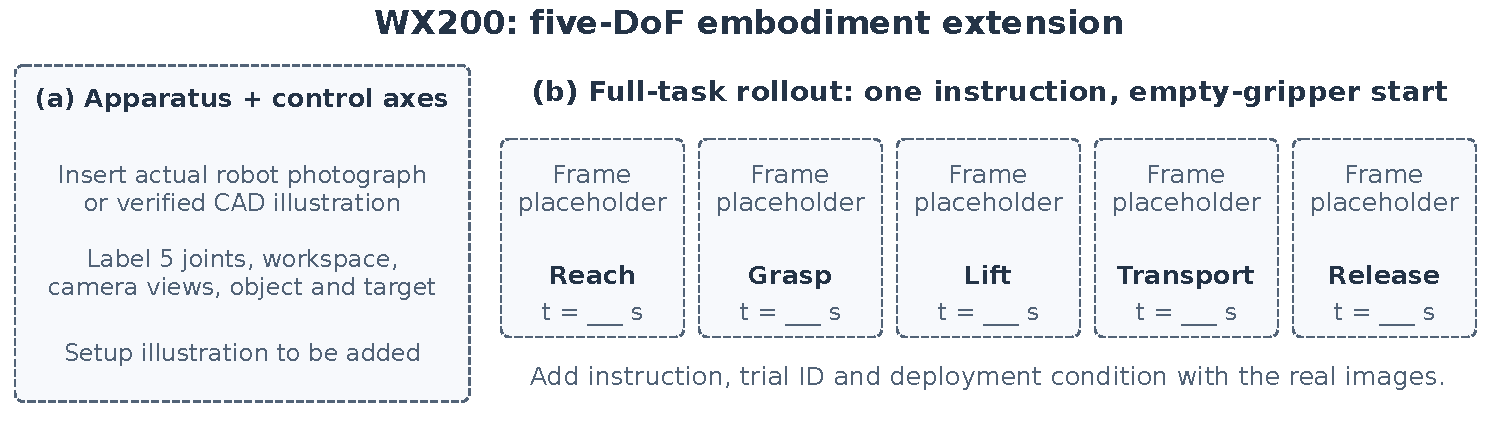
\includegraphics[width=\textwidth]{figures/wx200_slots.pdf}}
\caption{Reserved WX200 illustrations. (a) Five-DoF robot, workspace, cameras, and control-axis annotation. (b) Actual rollout frames for reach, grasp, lift, transport, and release. Add timestamps and the task instruction. The current panels are layout placeholders and contain no experimental evidence.}
\label{fig:wx200}
\end{figure*}

\subsection{Scope of the Evidence}
The complete-task result comes from one SmolVLA training lineage. The retention results summarize a small number of rounds, and the LIBERO results are descriptive endpoint comparisons. Neither study isolates every stage of the pipeline. Earlier assisted training is part of the inherited CDPR policy; the reported full-task evaluation uses no assistance.

